% Target: 35 pages
% Current: 3

\chapter{Adapters Effectivity in Machine Translation}
In this Chapter, we propose to use BERT and adapters for Machine Translation task. Specifically, we are interested to understand the effectivity of adapters when applied to the machine translation task by investigating different usage scenarios of adapters in sequence-to-sequence (\texttt{seq2seq}) framework. We conduct the experiments by separating them into three different areas:
\begin{itemize}
    \item Use BERT weights\footnote{We use publicly available BERT weights from Huggingface hub \url{https://huggingface.co}} as the pre-train weights and investigate the importance of adapters in encoder or decoder.
    \item Use BERT weights and investigate the importance of the pre-trained models in the encoder or decoder while fine-tuning with adapters and setting the weights of the opposite side with random numbers.
    \item Down-scaling BERT weights by either zeroing out some elements in BERT (\texttt{zbert}) or completely removing them from the weight matrix (\texttt{zsbert}).
\end{itemize}

\section{Fixed Variable Parameters of Experients}
\subsection{Framework}
\begin{table}[]
    \centering
    \begin{tabular}{@{}cc@{}}
        \toprule
        \textbf{Name}            & \textbf{Value}        \\ \midrule
        \textbf{Batch size}      & 64                    \\
        \textbf{Learning rate}   & 0.0005                \\
        \textbf{Vocabulary size} & 31102 (de), 30522(en) \\ \bottomrule
    \end{tabular}
    \caption{Fixed hyperparameters throughout the experiments}
    \label{tab:hyp_invest}
\end{table}

As we mentioned on tkhe beginning of the chapter, we have several scenario we use to conduct the experiments. Despite various possibilities of different setup, here we describe variables that we fixed throughout the experiments. As we have mentioned on Chapter 3 (**change this to ref**), we use Huggingface as our main framework with added modification for adapters. In contrary to Chapter 4 (**change this to ref**), we do not investigate language models that we train ourselves, but instead, we focus mainly on BERT language model. We use the same hyperparameters to Chapter 3(**change this to ref**) which we describe on Table \ref{tab:hyp_invest}


\subsection{Dataset}
As mentioned on the previous Section, in this experiment we no longer focus on the language model and instead we focus mainly on the machine translation. We have already described on Chapter 3 (**change this to ref**) that WMT is mainly used for language model training and mixed training for models that were trained from scratch. For machine translation, we use exclusively on IWSLT for our fine-tuning and evaluation stage.


\section{Original BERT}
\subsection{Size of adapters}
\subsubsection{Experiment setup}
\paragraph{}
In this experiments, we are keeping the rest of the parameters the same for all the models. The only parameter that we modify is the size of reduction ratio in the adapters. If we recall, adapters are bottleneck layers that will reduce the input size dimension before scaling it back. The definition of reduction ratio here translates to the number of dimension that we reduce within the bottleneck layer. To be more precise, if we use ``16'' as the reduction ratio, this means we are reducing the original layers by ``16'' and then scale it back to the original size.

We are using a various size of reduction ratio to compare the result. The purpose of this reduction is to see whether we can see further benefit in enlarging the adapters bottleneck size in term of performance. For this experiments, we use 16, 8, 4, 2, 1 as the ratio values. We compare the results with the baseline BERT that we fine-tuned by only modifying the cross-attention layer. We will refer this baseline as baseline BERT for the entirety of this work.

\subsubsection{Experiment results}
In this section, we are comparing the results of the baseline BERT with models that fine-tuned with adapters in different reduction ratios. For the baseline BERT model, we only fine-tuned the cross-attention layers and keep the rest of the weights impact. This is to understand whether we can gain benefit in just fine-tuning the cross-attention layer. We can see from Figure \ref{img:adapt_bert_ratio} that even the smallest model (\texttt{adapt\_bert\_reduc\_16}) can already outperform the baseline by around 2 BLEU. This shows that the adapters can help further improve the model's performance by adding only a small amount of weights during the fine-tuning.

\begin{figure}[]
    {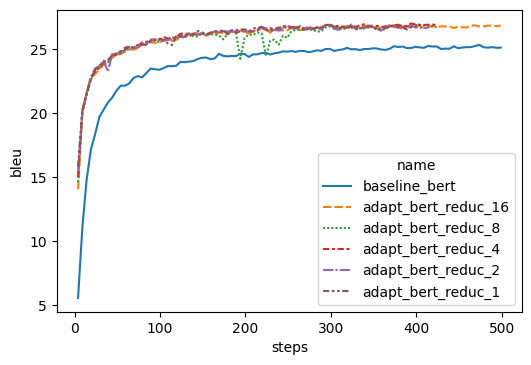
\includegraphics[width=0.95\textwidth]{img/adapter_bert_baseline_adapters.png}}
    \centering
    \caption{Comparison between baseline BERT model and adapters model with different ratio (16, 8, 4, 2, 1).}
    \label{img:adapt_bert_ratio}
\end{figure}

Furthermore, the difference between the ratios is pretty minimal. It suggests that there is not much benefit in expanding the size of adapters for the normal size BERT. It is possible that it is no longer trivial to append adapters to fine-tune the model for large-sized models such as the original BERT. Further improvement may be required to handle the different nature of BERT's output as it is naturally different from the normal machine translation objective such as auto-regression.

\subsection{Position of adapters (encoder vs decoder)}
\subsubsection{Experiment setup}
We would like to see the importance of adapters when put in different place. Since in this work we are working with sequence-to-sequence architecture, we would like to see whether only incorporating adapters on one side can already beneficial and hence reducing the weights addition to the model.

\subsubsection{Experiment result}
\label{sec:posadares}
\begin{figure}[]
    {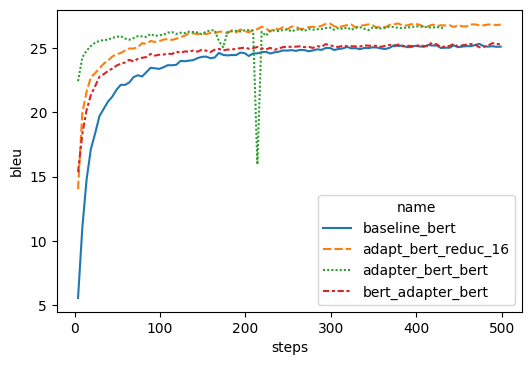
\includegraphics[width=0.95\textwidth]{img/bert_pos.png}}
    \centering
    \caption{Comparison between baseline BERT model and adapters model where the adapters are placed in three different setups: 1) Adapters in both encoder and decoder (\texttt{adapt\_bert\_reduc\_16}); 2) Adapters only in encoder (\texttt{adapter\_bert\_bert}); 3) Adapters only in decoder (\texttt{bert\_adapter\_bert}).}
    \label{img:adapt_bert_pos}
\end{figure}
We can see from Figure \ref{img:adapt_bert_pos} that by just adding the adapters on the encoder part, we see an improvement and outperform the baseline model. By adding the adapters on the encoder only, we can see that the model eventually achieved similar performance as if we added the adapters on both sides. For the decoder, on the other hand, we can see that there is no benefit in adding the adapters as there is no improvement in terms of BLEU compared to the baseline.

Adding the adapters on the encoder and fine-tuning it is more cost-effective than the decoder. With this finding, we can reduce the cost of fine-tuning by half when we do not include the adapters on the decoder.

\subsection{BERT in encoder vs decoder}
\subsubsection{Experiment setup}
In this section, we would like to see the importance of having the pre-training models as the initial weights in either the encoder or decoder. In addition to that, we also expand the experiment further by trying to understand the correlation of adding adapters on top of the randomly set weights.

We start by defining the definition of the setup in this experiments. In the previous Chapter, we have already introduced randomly set experiment where we instantiate the base Transformer model with only random weights. We then fine-tune the base Transformer model by only updating the adapters and cross-attention layer. In this setup, we are doing experiments in similar concept except that we only initialized the random weights on either the encoder and decoder. We then perform similar setup as in the Chapter xxx (position of adapters) where we put the adapters only in the encoder or decoder.

The purpose of the experiments are:
\begin{itemize}
    \item We want to understand further the importance of the pre-training model when fine-tuned with adapters. By initializing the model with BERT only in one component, we can see whether it is necessary to use BERT on both components when adapters are incorporated.
    \item We want to understand the capability of adapters when either one of the components do not contain useful information (relative to BERT). We would like to see whether the adapters can recover or even outperform some of the performance that we have already gathered from the previous chapters and sections.
\end{itemize}

\subsubsection{Experiment results}
This section compares models that use adapters in both encoder and decoder, only in the encoder and only in the decoder while only initializing either the encoder or decoder with BERT and the counterparts with a random set of weights. The purpose of the experiments is to understand the behaviour of adapters when faced with relatively poor representation in of the components.

\paragraph{Randomly set weights on encoder}
In this part of the section, we want to answer the main question: "To what extent can the adapters restore the missing gap when the encoder does not contain useful information (relative to BERT)?"

\begin{figure}[h]
    {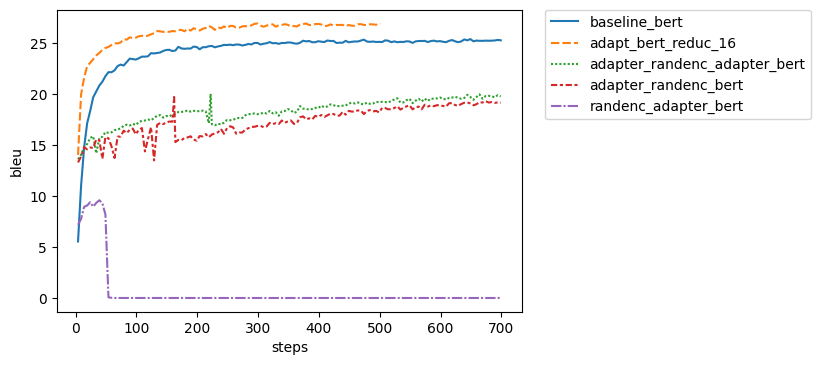
\includegraphics[width=0.95\textwidth]{img/adapter_bert_randenc.png}}
    \centering
    \caption{Comparison between baseline BERT model and adapters model where the adapters are placed in three different setups: 1) Adapters in both encoder and decoder (\texttt{adapt\_bert\_reduc\_16}); 2) Adapters only in encoder (\texttt{adapter\_bert\_bert}); 3) Adapters only in decoder (\texttt{bert\_adapter\_bert}) and the decoder is initialized with BERT while the encoder is initialized with random numbers.}
    \label{img:adapt_bert_randenc}
\end{figure}

We can see from Figure \ref{img:adapt_bert_randenc} that when adapters are appended in both components, we get to almost 20 in the BLEU score. This is relatively higher than the other two setups (adapters only in the encoder and adapters only in the decoder). However, compared to the baseline, we are missing 4 points in BLEU when we set the weights on the encoder as entirely random. This means that the base encoder model missing relatively essential information that the adapters can not simply restore during the fine-tuning.

We further focus on the adapters' performance compared to the baseline model that is only fine-tuned on the cross-attention layer to see whether there is any benefit in using adapters or simply fine-tuning the cross-attention is enough. We can see that the model that was only fine-tuning the cross-attention layer can not learn at all, while the adapters can perform significantly better. This marks the capability of the adapter when faced with a randomly set encoder.

When the adapters are removed from the decoder, we see a degradation in performance in about 1 BLEU. However, when the adapters are removed from the encoder, we can see the performance is completely depleted during the training. We also see the same behaviour in the next section when the weights on the decoder are set randomly. This tells us that there is some incompatibility in the weights (random and BERT) where it is not trivial to fine-tune the cross-attention layer without further adjustment to the base model's weights.

\paragraph{Randomly set weights on decoder}
Similar to the previous section, the main question in this experiment is, "To what extent can the adapters restore the missing gap when the decoder does not contain useful information (relative to BERT)?"

In contrast to when the randomly set weights are on the encoder side, we can see from Figure \ref{img:adapt_bert_randdec}, that the model has a close performance to the one we have on the BERT baseline. This tells us that the pre-training weights in the encoder are more critical than in the decoder when we have adapters on both sides. However, when removing the adapters on the encoder side, we see similar performance as in the previous section, where the performance drops to zero in the middle of training. This furthers our arguments that adapters are necessary to adjust the weights in the model so that the cross-attention layer can work properly.

\begin{figure}[h]
    {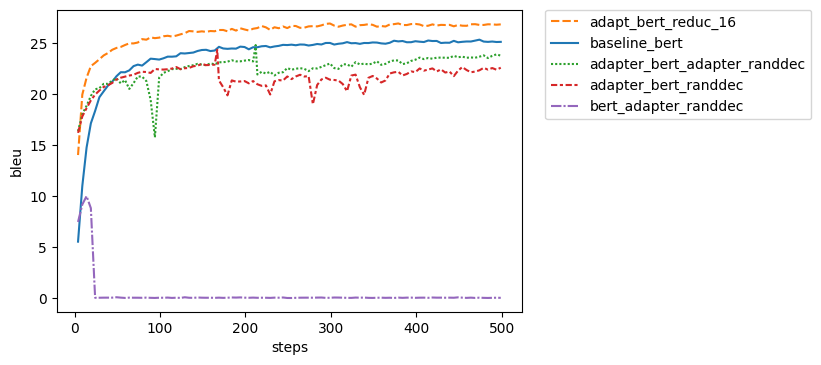
\includegraphics[width=0.95\textwidth]{img/adapter_bert_randdec.png}}
    \centering
    \caption{Comparison between baseline BERT model and adapters model where the adapters are placed in three different setups: 1) Adapters in both encoder and decoder (\texttt{adapt\_bert\_reduc\_16}); 2) Adapters only in encoder (\texttt{adapter\_bert\_bert}); 3) Adapters only in decoder (\texttt{bert\_adapter\_bert}) and the encoder is initialized with BERT while the decoder is initialized with random numbers.}
    \label{img:adapt_bert_randdec}
\end{figure}

On the other hand, when we remove the adapters from the decoder side, we can see that the performance is not as bad as when the adapters are removed from the encoder, but we still see a reduction in performance. We see around $<$ 1 BLEU when the model reaches 400k steps in the training stage.

\section{BERT size reduction}
\subsection{Zeroing columns}
\subsubsection{Experiment setup}
In this experiment, we will focus on soft reduction of BERT weights by zeroing the weights on every even index columns and rows in both Transformer body as well as in the embedding weights. The way we set this experiments by first manually editing the weights from BERT offline and then use the weights as the pre-trained models that later we will fine-tune using adapters. We further refer this setup as \texttt{zbert} for the rest of this writing.

Other than removing the columns, we also experimenting similar to Section xxx by initializing the adapters either on the encoder or the decoder. The goal of this particular experiments is to understand the behaviour of the model when the pre-trained models are replaced with this particular setup.

\subsubsection{Comparison with BERT baseline (full BERT fine-tuning)}
We first compare the \texttt{zbert} model without adapters and only fine-tuning the cross-attention layers. We use \texttt{zbert} weights on both encoder and decoder so that it is comparable to the model that uses full-weight BERT. We use the full-weight BERT as the baseline in this experiment.

\begin{figure}[]
    {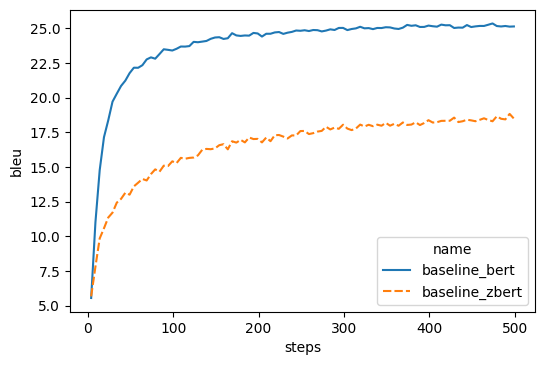
\includegraphics[width=0.95\textwidth]{img/baseline_zbert.png}}
    \centering
    \caption{Comparison between baseline BERT model and baseline \texttt{zbert} models.}
    \label{img:baseline_zbert}
\end{figure}

\begin{figure}[]
    {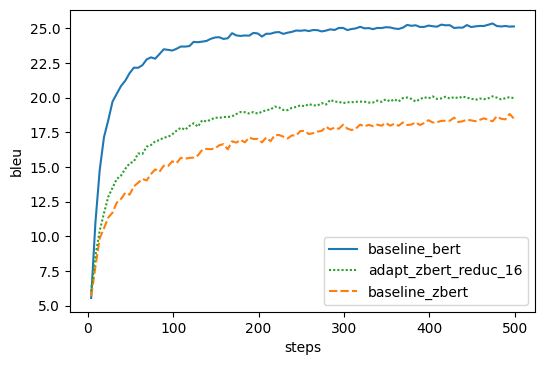
\includegraphics[width=0.95\textwidth]{img/adapter_zbert.png}}
    \centering
    \caption{Comparison between baseline BERT model, baseline \texttt{zbert} and adapters \texttt{zbert} models.}
    \label{img:adapter_zbert}
\end{figure}

We can see in Figure \ref{img:baseline_zbert} that we are losing performance of about 4 BLEU. This is quite significant as we are losing various essential features from the original BERT model. To see whether we can recover some of the performance with adapters, we continue our experiment by fine-tuning \texttt{zbert} model that is instantiated on both encoder and decoder sides with adapters. We can see from Figure \ref{img:adapter_zbert} that we only managed to recover 1 BLEU with a reduction ratio of 16.

\begin{figure}[]
    {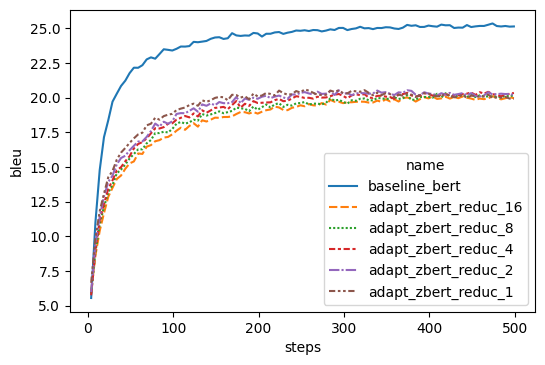
\includegraphics[width=0.95\textwidth]{img/adapter_zbert_ratio.png}}
    \centering
    \caption{Comparison between baseline BERT model and different reduction ratio of \texttt{zbert} models.}
    \label{img:adapter_zbert_ratio}
\end{figure}

From Figure \ref{img:adapter_zbert_ratio}, when we increase the size of the reduction ratio, initially, we can see some improvement compared to the higher ratio. However, they eventually converge to a similar performance by the end of training with no significant difference between different ratios. From this result, we can understand that depending on the base pre-trained model, adapters still have a limitation in achieving certain performance.

\paragraph{Adapters position}
In this section, we are trying to understand whether the position of both adapters and the pre-training models affect the model performance, similar to what we have seen in Section \ref{sec:posadares}. We use a similar setup as in the previous section, with the exception that we use \texttt{zbert} as the pre-trained model instead of the original BERT model.

\begin{figure}[h]
    {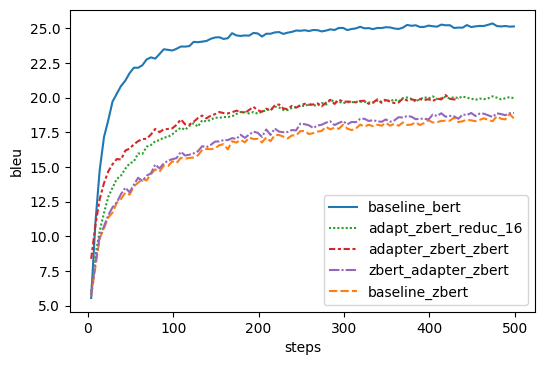
\includegraphics[width=0.95\textwidth]{img/zbert_pos.png}}
    \centering
    \caption{Comparison between baseline BERT model, baseline \texttt{zbert} model, adapters in both encoder and decoder of \texttt{zbert} model (\texttt{adapt\_zbert\_reduc\_16}), adapters only in encoder of \texttt{zbert} model (\texttt{adapter\_zbert\_zbert}), and adapters only in decoder of \texttt{zbert} model (\texttt{zbert\_adapter\_zbert}).}
    \label{img:zbert_pos}
\end{figure}

We can see from Figure \ref{img:zbert_pos} that when we include adapters on both encoder and decoder, we can outperform the baseline \texttt{zbert} in around 2 BLEU points. This shows that similar to the models that use BERT as the pre-training models, the adapters can help to improve the performance further even though some of the information is already missing in the base model.

Furthermore, we can also see that similar to the BERT model that was fine-tuned with adapters, using adapters only on the encoder side performs much better than on the decoder side. Other than that, we can also see that incorporating adapters only on the encoder side helps the model achieve better performance faster than the model that uses adapters on both sides. This further support our hypothesis that updating the representation on the encoder side is more beneficial. Looking deeper at the model with adapters on the decoder side, the performance is close to the baseline model, where we only fine-tune the cross-attention layer. This could mean that fine-tuning the decoder may not be enough to achieve better performance when the representation from the source side is constant.

\subsection{Model downscaling}
\subsubsection{Experiment setup}
This experiment is the continuation from \texttt{zbert} where we zeroing out some of the matrix elements. Specifically, instead of just zeroing out the elements, we now completely removing those elements from the matrix. The way we do this is similar to the one we do on \texttt{zsbert}. We remove the matrix elements on every even columns and rows in both Transformer body as well as the embedding weights. We similarly do the weights processing offline before using it as the pre-training base model. For the rest of this writing, we refer to this setup as \texttt{zsbert}.

Furthermore, we also follow similar setup as in Section xxx where we experiment on the position of the adapters position. The goal of this experiments is that we would like to understand the behaviour of the model compared to the baseline as well as \texttt{zbert}.

\subsubsection{Comparison with BERT baseline and \texttt{zbert}}

\begin{figure}[h]
    {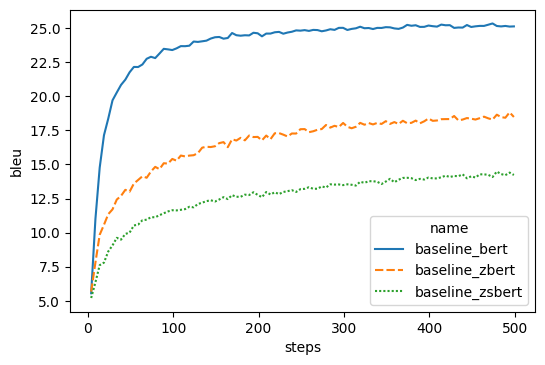
\includegraphics[width=0.95\textwidth]{img/baseline_zsbert.png}}
    \centering
    \caption{Comparison between baseline BERT model and baseline \texttt{zsbert} model.}
    \label{img:baseline_zsbert}
\end{figure}

\begin{figure}[]
    {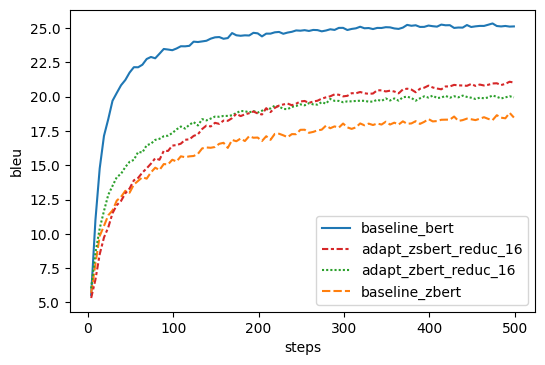
\includegraphics[width=0.95\textwidth]{img/adapter_zsbert.png}}
    \centering
    \caption{Comparison between baseline BERT model, baseline \texttt{zbert}, baseline \texttt{zsbert} and adapters \texttt{zsbert} models.}
    \label{img:adapter_zsbert}
\end{figure}

We begin with the comparison of \texttt{zsbert} with the BERT baseline. We can see from Figure \ref{img:baseline_zsbert} that the performance degrades significantly for almost 10 BLEU. This is also significantly worse than \texttt{zbert} where we only lose 5 BLEU. After some investigation, we realize that removing weights from the network is not straightforward as the computation of layer normalization layer in the transformer will compute different results as the normalization scaling factor will also be different. With manual evaluation, we found a slight difference between weights that were only zeroed and weights that are completely removed. Despite the small difference in the output of layer normalization, the error will be propagated to the top layers, causing the result to differ significantly.

From the challenge above, we are also interested to see whether adapters have the capability to mitigate the problem and able to recover some of the performance. We can see from Figure \ref{img:adapter_zsbert} that adapters with a 16 ratio already managed to improve the performance up to 6 BLEU. This shows another capability of adapters to intermediate numerical errors in the middle of the layers. We also notice a leap in final performance when we compare the adapter model with an equal reduction ratio (16) between \texttt{zbert} and \texttt{zsbert}. We can see that initially \texttt{zsbert} performs worse than \texttt{zbert}. After some steps, we can see the performance in \texttt{zbert} starting to stall but not in \texttt{zsbert}. We hypothesize this relates to a similar reason that we stated in the original BERT model, where we could not see any improvement when increasing the reduction ratio. It is possible that when we reduce the size of the original pre-trained model, the adapters manage to adjust the flow of information within the network and better replacing the missing information with new knowledge that is more important to solve the task.


\begin{figure}[]
    {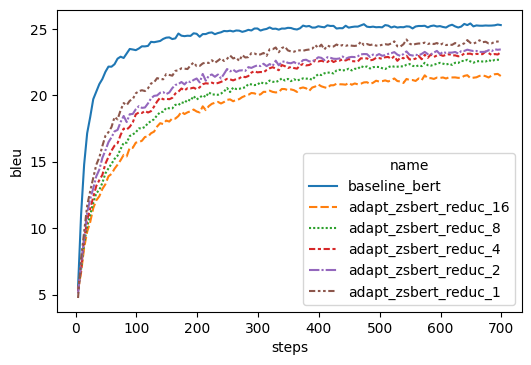
\includegraphics[width=0.95\textwidth]{img/adapter_zsbert_ratio.png}}
    \centering
    \caption{Comparison between baseline BERT model and different reduction ratio of \texttt{zsbert} models.}
    \label{img:adapter_zsbert_ratio}
\end{figure}

In Figure \ref{img:adapter_zsbert_ratio}, when the adapters reduction ratio is further reduced, we can see that the performance is also improving up to the point where it has the close performance to the baseline model. This remarks a prominent result as we can see from Table \ref{tab:numvars} that the total number of weights (including adapters) is reduced significantly.

\begin{table*}[]
    \centering
    \begin{tabular}{@{}cccc@{}}
        \toprule
        \textbf{Name}                                                               &
        \textbf{\begin{tabular}[c]{@{}c@{}}\# Trainable\\ Variables\end{tabular}}   &
        \textbf{\begin{tabular}[c]{@{}c@{}}\# Untrainable\\ Variables\end{tabular}} &
        \textbf{\begin{tabular}[c]{@{}c@{}}\# Total\\ Variables\end{tabular}}                                                \\ \midrule
        \textbf{Adapters ratio 16}                                                  & 7.736.826  & 95.143.296  & 102.880.122 \\
        \textbf{Adapters ratio 8}                                                   & 8.179.770  & 95.143.296  & 103.323.066 \\
        \textbf{Adapters ratio 4}                                                   & 9.065.658  & 95.143.296  & 104.208.954 \\
        \textbf{Adapters ratio 2}                                                   & 10.837.434 & 95.143.296  & 105.980.730 \\
        \textbf{Adapters ratio 1}                                                   & 14.380.986 & 95.143.296  & 109.524.282 \\
        \textbf{Normal BERT}                                                        & 28.990.078 & 218.819.328 & 247.809.406 \\ \bottomrule
    \end{tabular}
    \caption{Total trainable variables in \texttt{zsbert} with adapters on different ratio vs normal BERT model}
    \label{tab:numvars}
\end{table*}

\subsubsection{Adapters position}

\begin{figure}[h]
    {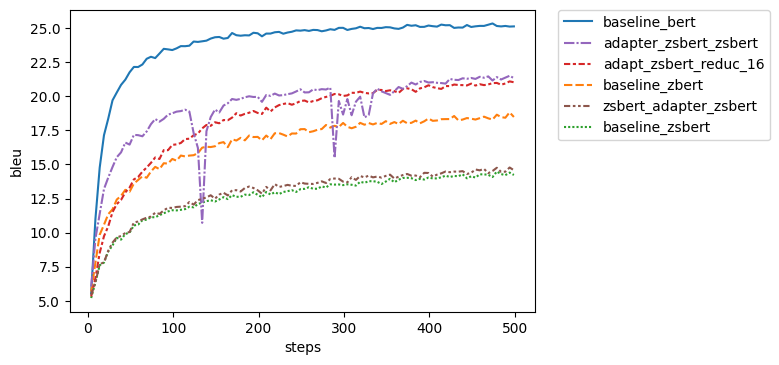
\includegraphics[width=0.95\textwidth]{img/zsbert_pos.png}}
    \centering
    \caption{Comparison between baseline BERT model, baseline \texttt{zsbert} model, adapters in both encoder and decoder of \texttt{zsbert} model (\texttt{adapt\_zsbert\_reduc\_16}), adapters only in encoder of \texttt{zsbert} model (\texttt{adapter\_zsbert\_zsbert}), and adapters only in decoder of \texttt{zsbert} model (\texttt{zsbert\_adapter\_zsbert}).}
    \label{img:zsbert_pos}
\end{figure}

From Figure \ref{img:zsbert_pos}, similar to the \texttt{zbert} experiments, we can see similar behaviour as models that are fine-tuned with adapters outperform the baseline \texttt{zsbert} and \texttt{zbert} models. Compared to \texttt{zbert} experiments, we notice a bigger gap in performance improvement in \texttt{zsbert}. In \texttt{zbert}, the difference between baseline and adapters is in the range of 5 BLEU. On the other hand, in \texttt{zsbert} we see the improvement is in the range of 8 BLEU. This result is particularly interesting for us as we recall from the baseline experiments that due to the numerical error from the layer normalization, we expect the difference is similar to \texttt{zbert} and have lower performance than we currently have. To further deep-dive on this, we refer to Figure \ref{img:zbert_vs_zsbert} to show the comparison between adapters in \texttt{zbert} and \texttt{zsbert}. We compare the adapters model with equal reduction ratio (16) between these two setup. We can see that initially \texttt{zsbert} performs worse than \texttt{zbert}. After some steps, we can see the performance in \texttt{zbert} starting to stall but not in \texttt{zsbert}. We hypothesize this relates to similar reason that we state on the original BERT model where we could not see any improvement when we increase the reduction ratio. It is possible that when we reduce the size of the original pre-trained model, the adapters manage to adjust the flow of information within the network and better replacing the missing information with new knowledge that is more important to solve the task.

\begin{figure}[h]
    {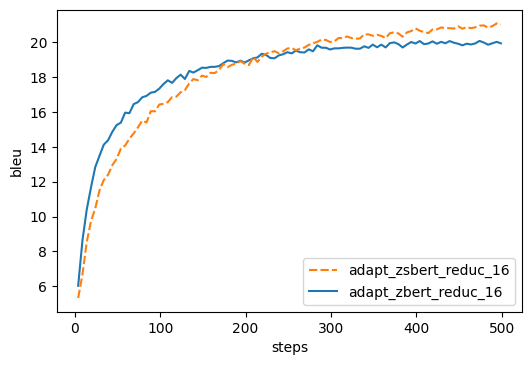
\includegraphics[width=0.95\textwidth]{img/zbert_vs_zsbert.png}}
    \centering
    \caption{Comparison adapters performance in \texttt{zsbert} and \texttt{zbert}. Both are using reduction ratio 16 and the adapters are placed on encoder and decoder.}
    \label{img:zbert_vs_zsbert}
\end{figure}

We see similar behaviour as we see on \texttt{zbert} experiments in regards of the position of the adapters. In Figure \ref{img:zsbert_pos}, the benefit of incorporating adapters on the encoder side is also apparent and outperform the decoder counterpart. We can also see a similar behaviour where eventually the performance of model with adapters on encoder outperform model with adapters on both side. Furthermore, we also see similar behaviour as in \texttt{zbert} for models with adapters where the performance is very close to the baseline and not improving as much as the encoder side. We hypothesize the same reason as we have stated in \texttt{zbert} could apply in \texttt{zbert} as well. Essentially, we need to modify the representation on the encoder side in order to achieve better performance.